Para verificar el correcto funcionamiento del sistema que hemos creado, hemos llevado a cabo pruebas con distintas plantillas de informe basadas en DICOM-SR para comprobar que la funcionalidad del sistema que hemos desarrollado.\par
A modo de ejemplo en este capítulo veremos cómo funciona el sistema, utilizaremos el fichero XML que contine una plantilla  basada en DICOM-SR que podemos encontrar en el apéndice \ref{dicom-sr-template}, y en los siguientes apartados comprobaremos como a partir de este fichero obtenemos una aplicación Android. \par

\lstset{escapechar=@,style=dicom}

\section{Análisis sintáctico de un informe plantilla basado en DICOM-SR}
En primer lugar realizamos el análisis sintáctico del fichero XML que contiene la plantilla del informe médico estructurado basado en DICOM-SR.\par
Tras este proceso tendremos cargada en memoria los datos relativo a la plantilla DICOM-SR en una estructura de datos arbórea. Al imprimir esta estructura de datos por consola, que podemos ver en el ejemplo de código \ref{ver:dicomTree}, comprobamos que la información contenida en el árbol es la misma que la que contenía el fichero XML de entrada. \par

\begin{lstlisting}[label=ver:dicomTree,caption=Registro del informe DICOM-SR cargado en  memoria]

  -------  EXPORACIÓN DE MAMA ---------- 

 - [SNOMED_CT_172117008] EXPLORACIÓN  DE LA MAMA 
 |   - date: Fecha Informe
 |   - text: Identificador
 |   - text: Identificador del Paciente
 ----- [RADLEX_RID29896] MAMA DERECHA 
 --------- [TRENCADIS_MAMO_TRMM0009] MASA 
 |           - text: Identificador 
 |           - num: Cuadrante Supero-Externo (CSE) de la Mama Derecha 
 |           - num: Cuadrante Infero-Externo (CIE) de la Mama Derecha 
 |           - num: Cuadrante Supero-Interno (CSI) de la Mama Derecha 
 |           - num: Cuadrante Infero-Interno (CII) de la Mama Derecha 
 |           - num: Línea Intercudrántica Externa (LIE)
 |           - num: Línea Intercuadrántica Superior (LIS)
 |           - num: Línea Intercudrántica Inferior (LIInf)
 |           - num: Línea Intercudrántica Interna (LIInt) 
 |           - num: Retroareolar de la Mama Derecha
 |           - num: Pezón de la Mama Derecha
 |           - num: Areola de la Mama Derecha
 |           - num: Prolongación Axilar de la Mama Derecha
 |           - num: Axila de la Mama Derecha 
 |           - num: Surco Inframamario de la Mama Derecha
 |           - num: Surco Intermamario de la Mama Derecha
 ----- [RADLEX_RID29897] MAMA IZQUIERDA 
 --------- [TRENCADIS_MAMO_TRMM0010] ASIMETRIA 
 |           - text: Identificador
 |           - num: Cuadrante Supero-Externo (CSE) de la Mama Izquierda
 |           - num: Cuadrante Infero-Externo (CIE) de la Mama Izquierda
 |           - num: Cuadrante Supero-Interno (CSI) de la Mama Izquierda
 |           - num: Cuadrante Infero-Interno (CII) de la Mama Izquierda
 |           - num: Línea Intercudrántica Externa (LIE) 
 |           - num: Línea Intercuadrántica Superior (LIS) 
 |           - num: Línea Intercudrántica Inferior (LIInf)
 |           - num: Línea Intercudrántica Interna (LIInt) 
 |           - num: Retroareolar de la Mama Izquierda 
 |           - num: Pezón de la Mama Izquierda 
 |           - num: Areola de la Mama Izquierda
 |           - num: Prolongación Axilar de la Mama Izquierda
 |           - num: Axila de la Mama Izquierda
 |           - num: Surco Inframamario de la Mama Izquierda 
 |           - num: Surco Intermamario de la Mama Izquierda 
\end{lstlisting}

Con el informe cargado en memoria es el momento de pasar a la generación de los ficheros necesarios para crear una aplicación Android para el informe estructurado.\par


\section{Generación automática de una aplicación Android}
Disponemos de una aplicación Android, cuya estructura hemos visto en \ref{tree:AndroidFramewok}. Esta aplicación carece del contenido necesario para un informe concreto, para completarla necesitamos el código que generamos mediante la aplicación Python que hemos desarrollado.\par
Como hemos explicado en apartados anteriores generaremos los ficheros necesarios para crear la vista, el modelo y el controlador de una aplicación Android. Para lograrlo recorremos el árbol que contiene la información del informe estructurado de entrada y vamos generando el código de la aplicación. Poodemos ver los ficheros que hemos creado en la figura \ref{ver:ficheros}.\par

\begin{figure}
\centering
\framebox[1.05\textwidth]{%
\begin{minipage}{0.95\textwidth}
	\dirtree{%
		.1 \textbf{outputs}/.
		.2 \textbf{activities}/.
		.3 Summary\_snomed\_ct\_172117008.java .
		.3 Tree\_snomed\_ct\_172117008\_radlex\_rid29896.java .
		.3 Tree\_snomed-ct\_172117008\_radlex\_rid29897.java .
		.3 Edit\_radlex\_rid29897\_trencadis\_mamo\_trmm0010.java.
 		.3 Edit\_radlex\_rid29896\_trencadis\_mamo\_trmm0009.java.
 		.3 Snomed\_ct\_172117008\_ListAdapter.java.
 		.2 \textbf{layouts}.
 		.3 tree\_snomed\_ct\_172117008\_radlex\_rid29897.xml.
 		.3 tree\_snomed\_ct\_172117008\_radlex\_rid29896.xml .
 		.3 summary\_snomed\_ct\_172117008.xml .
 		.3 edit\_radlex\_rid29897\_trencadis\_mamo\_trmm0010.xml.
 		.3 edit\_radlex\_rid29896\_trencadis\_mamo\_trmm0009.xml.
 		.2 \textbf{manifest}.
 		.3 AndroidManifest.xml.
 		.2 \textbf{model}/.
		.3 Snomed\_ct\_172117008\_radlex\_rid29897.java .
		.3 Snomed\_ct\_172117008\_radlex\_rid29897\_Children.java.
		.3 Snomed\_ct\_172117008\_radlex\_rid29897\_Group.java .
		.3 Snomed\_ct\_172117008\_radlex\_rid29896.java . 
		.3 Snomed\_ct\_172117008\_radlex\_rid29896\_Children.java.
		.3 Snomed\_ct\_172117008\_radlex\_rid29896\_Group.java .
		.3 Snomed\_ct\_172117008.java.
		.3 Radlex\_rid29897\_trencadis\_mamo\_trmm0010.java.
		.3 Radlex\_rid29896\_trencadis\_mamo\_trmm0009.java.
		.2 \textbf{strings}/.
		.3 strings\_es\_ES.xml .
		.3 strings.xml .
	}
\end{minipage}
}
\caption{Estructura de ficheros generados}
\label{ver:ficheros}
\end{figure}


\section{Aplicación Android para el informe de entrada}\label{sec:appfinal}

Todos los ficheros de código que hemos generado se integran mediante un sencillo script dentro de la aplicación esqueleto de Android, obteniendo una aplicación funcional en Android.\par

En las figura \ref{ver:summary} vemos la pantalla de inicio, en esta pantalla el usuario podrá introducir los datos del informe a la izquierda y a la derecha vemos los órganos que son estudiados en este informe (mama derecha y mama izquierda).\par


\begin{figure}[ht]
\centering
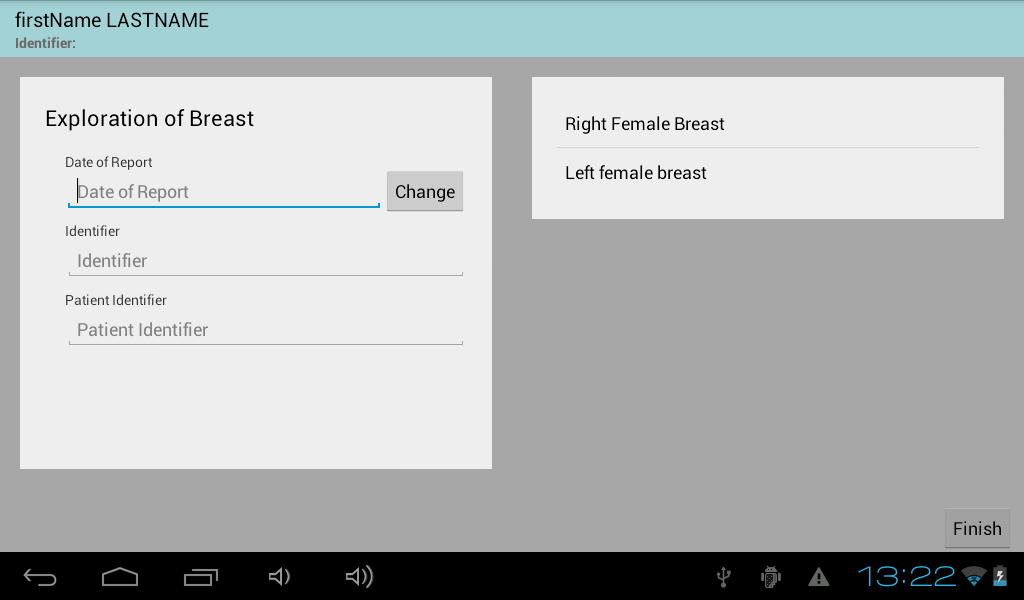
\includegraphics[scale=0.4]{./imgs/verificacion/summary.png}
\caption{Pantalla de inicio de la aplicación Android para una exploración de pecho}
\label{ver:summary}
\end{figure}

Si el usuario decide añadir una lesión en la mama derecha, el sistema le llevará a la pantalla que podemos ver en la figura \ref{ver:treeRFB}. Como en el fichero XML se define que la mama derecha sólo puede contener lesiones de tipo \emph{Masa}, vemos únicamente esta en el listado de lesiones de la mama derecha. El caso de la mama izquierda es análogo, sólo que en este caso en el infome hemos definido que la mama izquierda solamente puede contener lesiones de tipo \emph{Asimetrías}, vemos este ejemplo en la figura \ref{ver:treeLFB}.\par

\begin{figure}[ht]
\centering
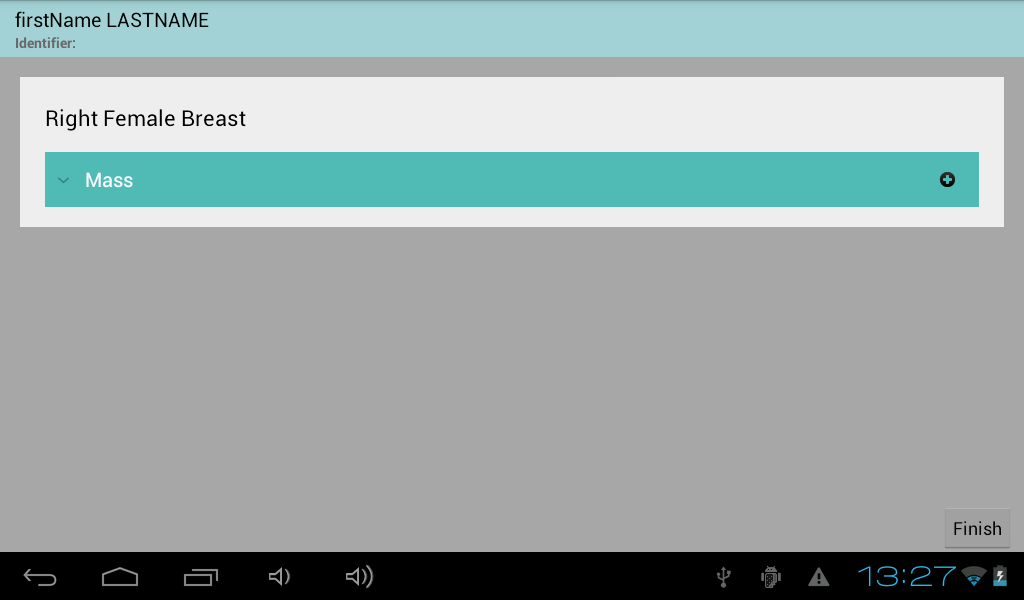
\includegraphics[scale=0.4]{./imgs/verificacion/treeRFB.png}
\caption{Lesiones de la mama derecha}
\label{ver:treeRFB}
\end{figure}

\begin{figure}[ht]
\centering
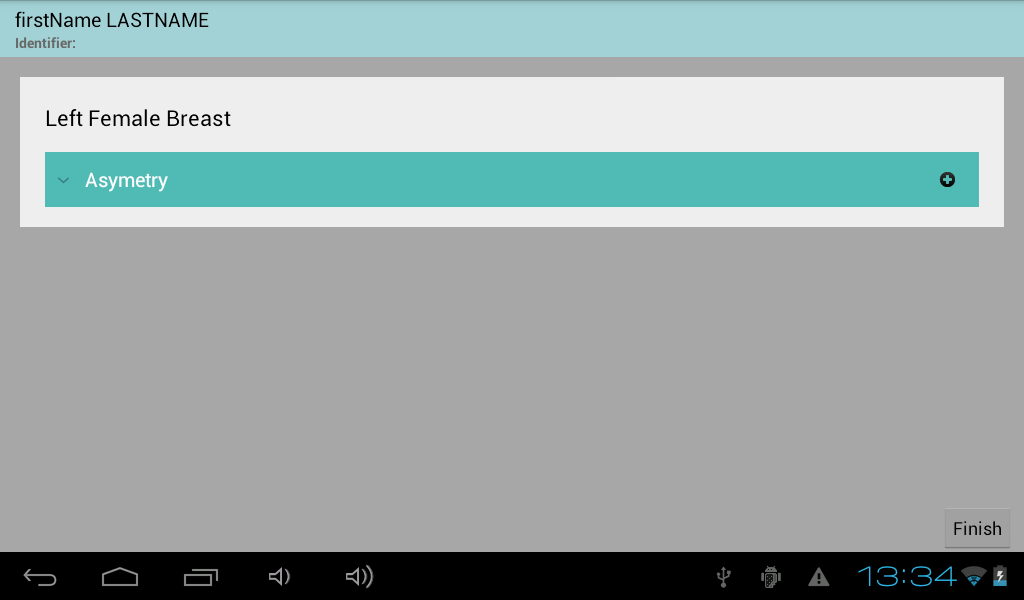
\includegraphics[scale=0.4]{./imgs/verificacion/treeLFB.png}
\caption{Lesiones de la mama izquierda}
\label{ver:treeLFB}
\end{figure}

Por último veremos las figura que permiten añadir y editar lesiones del informe. En la figura \ref{ver:editMass} vemos el ejemplo que permite añadir y editar lesiones de tipo \emph{masa}, mientras que en la figura \ref{ver:asymmetry} podemos ver la pantalla que nos permite añadir y editar lesiones de tipo \emph{asimetría}.\medskip\par


\begin{figure}[ht]
\centering
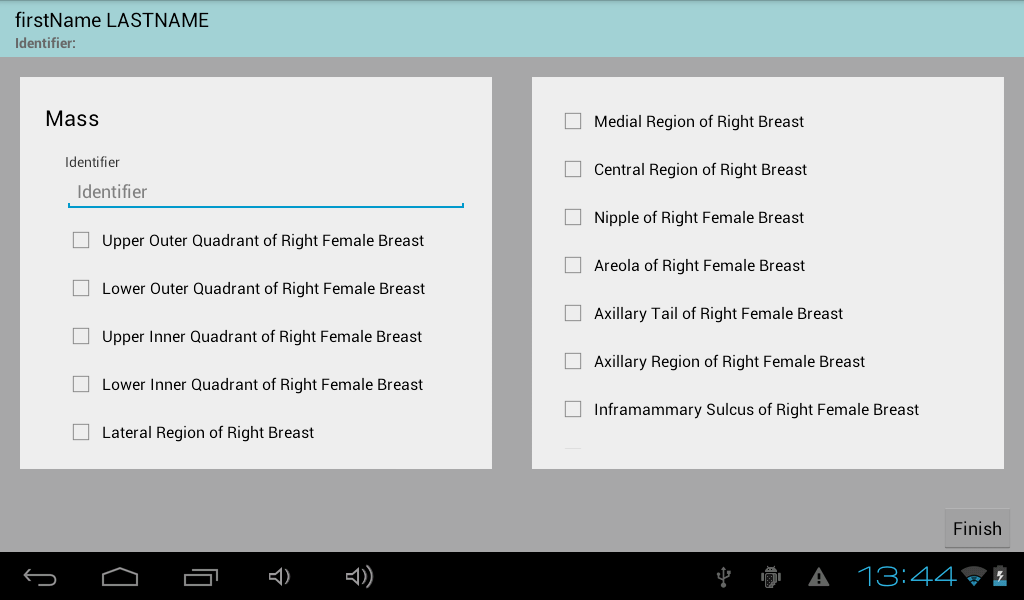
\includegraphics[scale=0.4]{./imgs/verificacion/editMass.png}
\caption{Añadir y editar una lesión de tipo masa}
\label{ver:editMass}
\end{figure}

\begin{figure}[ht]
\centering
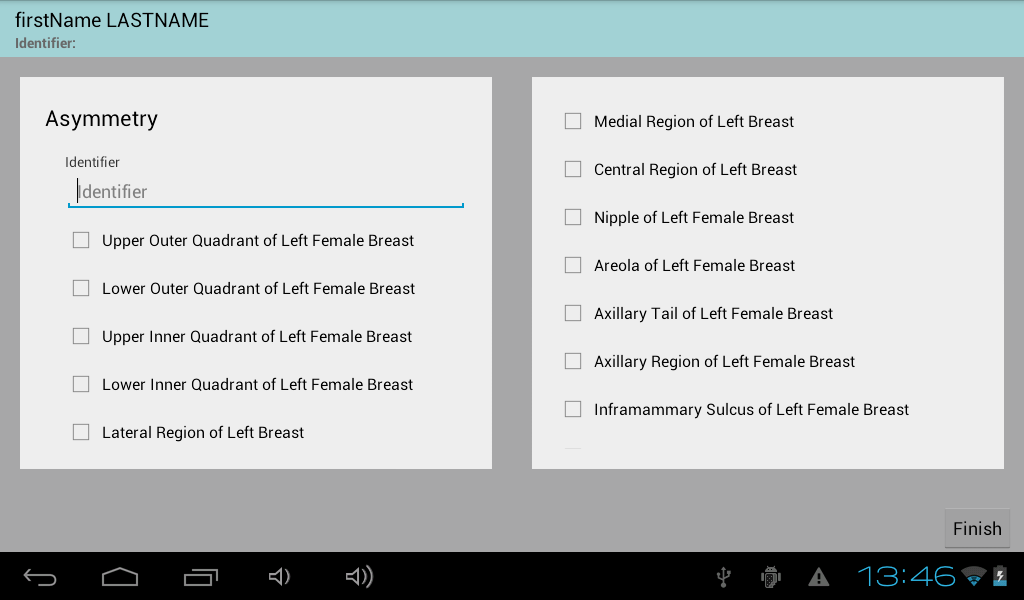
\includegraphics[scale=0.4]{./imgs/verificacion/asymmetry.png}
\caption{Añadir y editar una lesión de tipo asimetría}
\label{ver:asymmetry}
\end{figure}

Hemos seleccionado un informe estructurado médico bastante reducido, de modo que el tamaño de los documentos fuera razonable para incluirlos en esta memoria y contuviera todos los conceptos básicos para explicar el funcionamiento del sistema que hemos desarrollado.\par
De modo que al tratarse de un ejemplo sencillo la aplicación resultante también es sencilla. Pero el proceso que hemos descrito puede generalizarse y aplicarse a cualquier fichero XML plantilla basado en XML.